\documentclass[../../../main.tex]{subfiles}

\begin{document}

\section{IceCube, Cosmic Rays, and Neutrinos from Deep Space}
\label{sec:professional}

\textit{Cosmic rays} are high-energy protons, electrons, and nuclei propagating through space near the speed of light.  They carry information from other regions in the galaxy, and in some case, other galaxies.  Since the discovery of extremely energetic cosmic rays more than a half century ago, the quest to uncover their sources continues.  Despite progress in experimental capabilities and theoretical insight, we do not yet know the acceleration mechanism for those particles with energies that have been measured in excess of $10^{20}$ electron-volts \cite{10.1088/1742-6596/1766/1/012002}.  Being electrically charged, cosmic rays paths are curved by electromagnetic fields in space.  By the time the cosmic ray arrives at Earth, the arrival direction no longer points back to the origin.  In addition, interactions with cosmic microwave background (CMB) photons can block ultra-high energy cosmic rays from reaching Earth \cite{PhysRevLett.16.748} \cite{1966JETPL...4...78Z}.
\\
\vspace{0.15cm}
Neutrino astronomy offers a powerful tool to discover the physics associated with cosmic ray acceleration, which is not accessible with other \textit{messengers}: cosmic-rays, gamma-rays, and  optical photons. Charged cosmic rays which interact with gas, dust, or radiation near an accelerating object produce gamma-rays and high-energy neutrinos.  These neutrinos are called \textit{astrophysical} neutrinos. Whereas gamma-rays can be absorbed in dense environments, astrophysical neutrinos can escape and travel unimpeded to a detector (\cite{Astro2020_1} and references therein). Neutrinos travel at the speed of light in straight lines, undeflected by electromagnetic fields.  This allows for identification of sources, as well as the potential for finding sources that emit both neutrinos and gravitational waves \cite{10.3847/2041-8213/ab9d24}.
\\
\vspace{0.15cm}
The most energetic cosmic rays that do escape their source can interact with the cosmic microwave background en route to the Earth, generating cosmogenic neutrinos with a characteristic energy distribution peaking at $10^{18}$ electron-volts \cite{10.1007/bf00645585} \cite{BERESINSKY1969423}.  Neutrinos at these energies still do not interact with the CMB often enough to be blocked from arriving at Earth.  Neutrinos offer a window into regions of the Universe \textit{far beyond what is possible} with other messengers.  A flux of neutrinos originating outside the solar system with energies between $10^{13}$ and $10^{15}$ electron-volts has been measured by the IceCube collaboration \cite{PhysRevLett.111.021103}. Previous analyses have shown that the discovery of ultra-high energy neutrinos (UHE-$\nu$, energy greater than $10^{15}$ electron-volts) will require a detector with a larger volume because the flux decreases with energy \cite{PhysRevD.98.062003}. UHE-$\nu$ are the ones that could potentially explain the origin of cosmic rays.  UHE-$\nu$ also provide the chance to study quantum mechanical interactions never probed before \cite{Astro2020_1} \cite{Astro2020_2}.
\\
\vspace{0.15cm}
Utilizing the \textit{Askaryan effect}, in which UHE-$\nu$ creates a radio-frequency pulse, greatly expands the effective volume of UHE-$\nu$ detector designs.  This effect is important for UHE-$\nu$ detection, because radio pulses travel more than 1 kilometer in Antarctic and Greenlandic ice \cite{10.3189/2015jog14j214} \cite{10.3189/2015jog15j057} \cite{10.1002/2015rs005849} \cite{10.1016/j.astropartphys.2011.11.010}.  Stations can be placed 1 km apart, and the volume of the overall array of stations is large enough to capture UHE-$\nu$.  The large volume is necessary for two reasons.  First, cosmic rays and neutrinos at these energies are rare enough that a $10 \times 10$ km$^2$ target is necessary.  Second, neutrinos do not always interact in dense matter quantum mechanically, unlike protons or heavy ions.  To ensure that we record the UHE-$\nu$ that do interact, we must construct a large detector.

\subsection{Radio Expansions: IceCube Generation 2}
\label{sec:gen2}

\begin{figure}
\centering
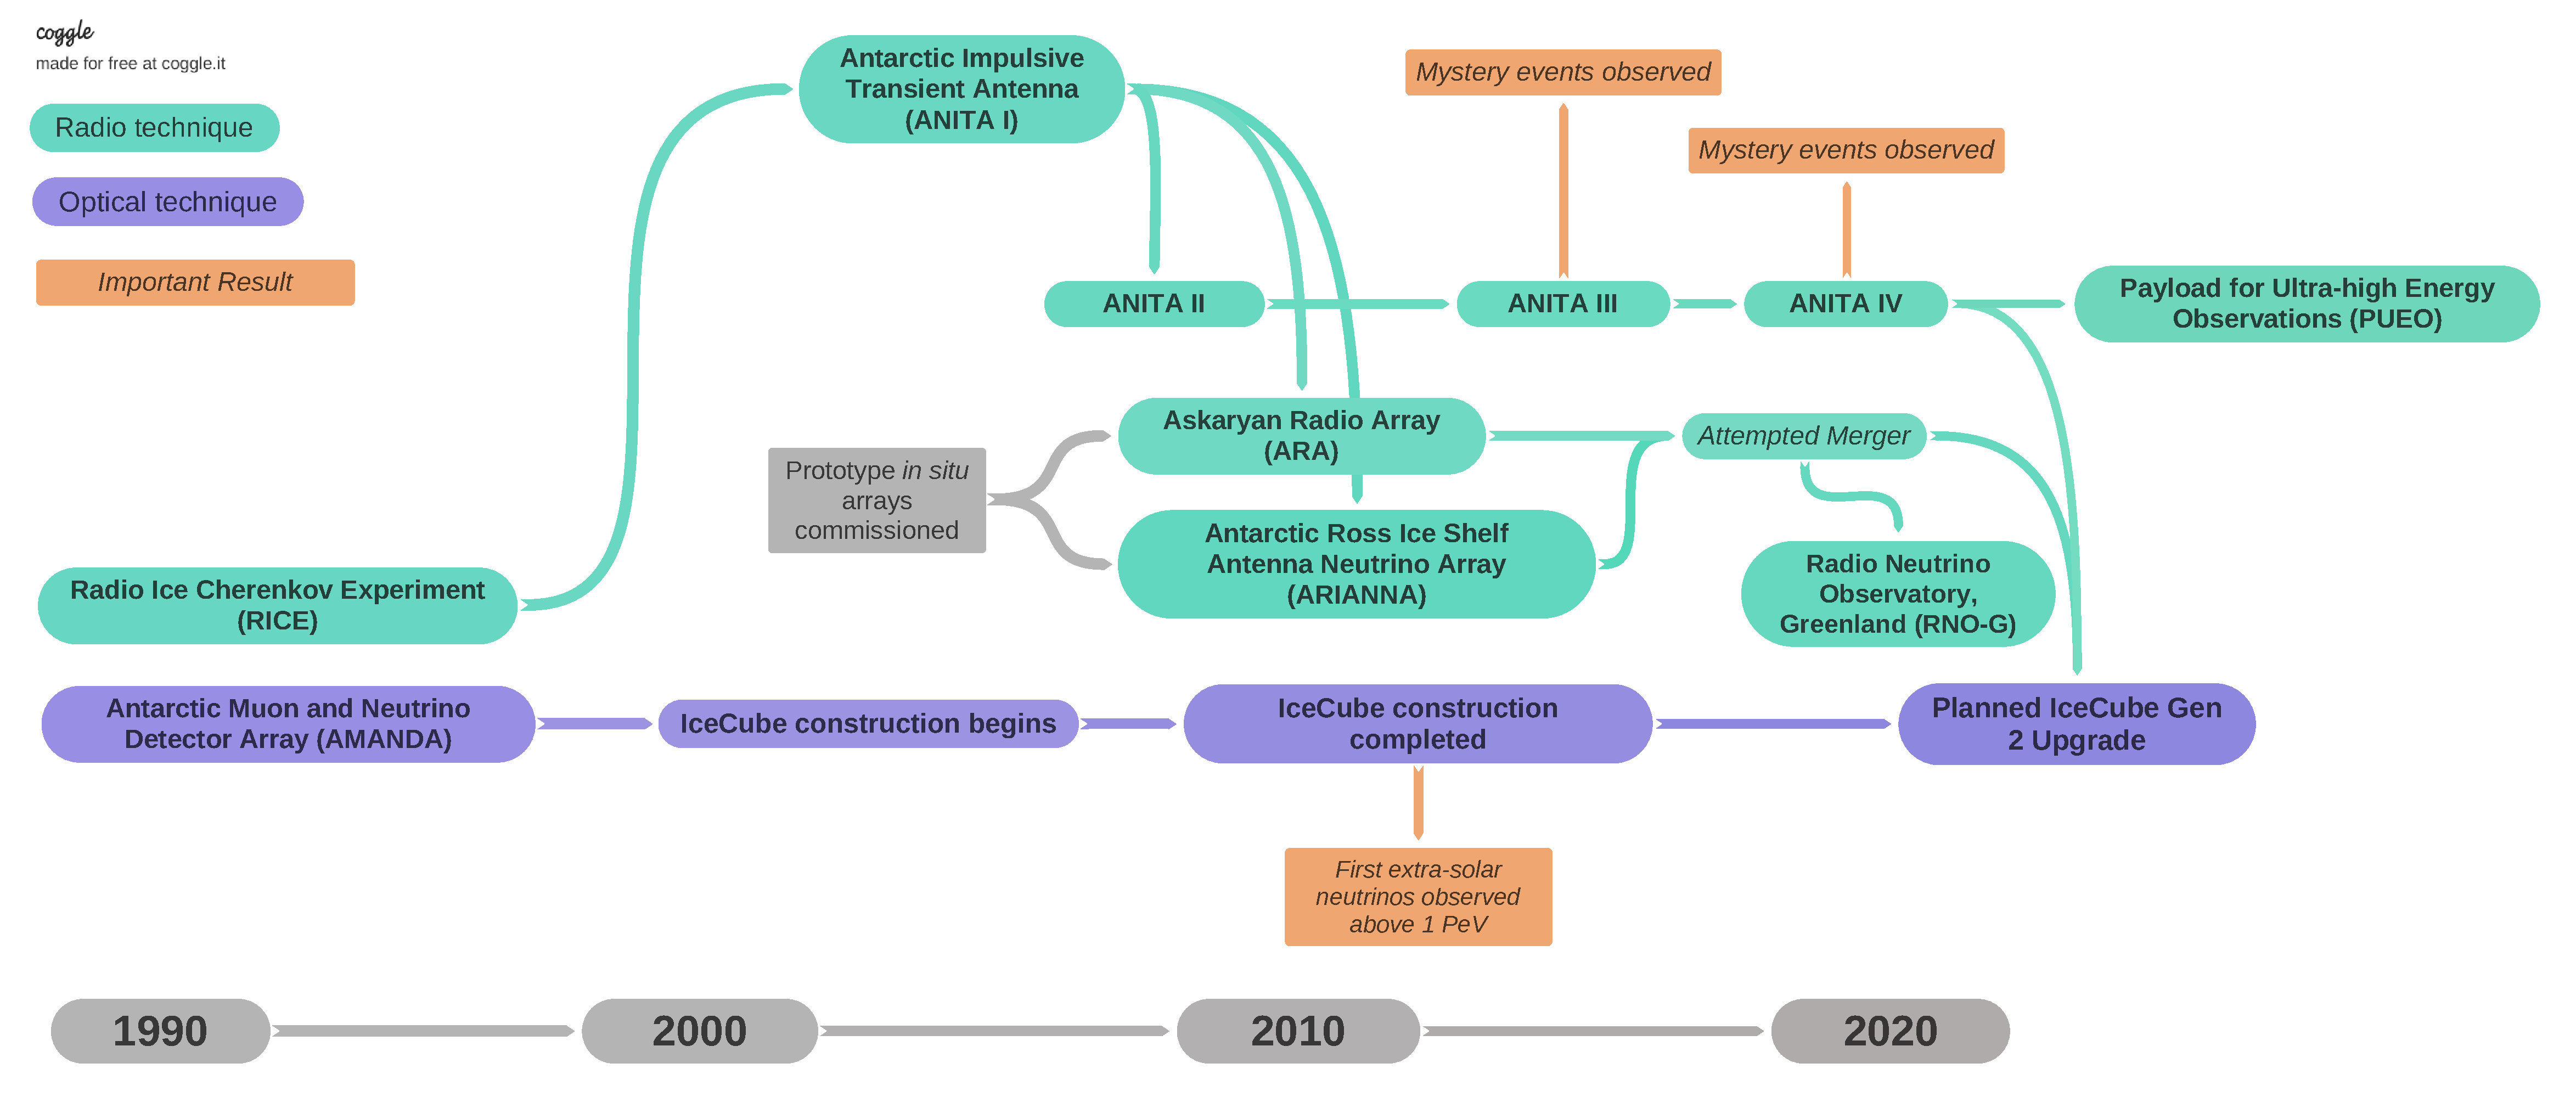
\includegraphics[width=\textwidth]{figures/timeline.pdf}
\caption{\label{fig:flow} A general timeline of the UHE-$\nu$ sub-field of physics.}
\end{figure}

In Sec. \ref{sec:origin}, I reflected on my academic origins.  The plot has taken an interesting and favorable turn for Whittier College.  The IceCube Collaboration finally recognized the necessity of radio-based detectors \cite{PhysRevD.98.062003}, and now includes components developed by ARIANNA.  Whittier College has been invited to become a member institution of The IceCube Collaboration through my scholarship, giving our students access to cutting-edge physics research.  I list the advantages in Sec. \ref{sec:invite} below.
\\
\vspace{0.15cm}
The diagram in Fig. \ref{fig:flow} illustrates progress made in the last decade.  IceCube is the largest neutrino detector in the world, and one of the more expensive physics projects in US history (\$0.28 billion).  In perspective, the Mars rover Curiosity cost \$2.5 billion, and the Advanced LIGO gravity-wave detector cost \$1.1 billion.  IceCube was built from a predecessor called AMANDA, constructed at the South Pole for the abundant, quality ice \footnote{Being at the South Pole is like being atop a 2.8 km ice mountain.  The ice thickness is needed to form the largest block of ice possible for the detector.}.  AMANDA and IceCube have relied on the \textit{optical technique}, observing tracks of optical photons left by neutrinos.  Practically, this limits the detector volume to 1 km$^3$, for optical photons only propagate $\approx 100$ m in ice.  After years of construction, IceCube announced the observation of \textit{extra-solar}\footnote{Originating from outside the solar system.} neutrinos with energies of $10^{15}$ electron-volts in 2013 \cite{PhysRevLett.111.021103}.  This result broke the world record for highest-energy neutrino ever observed by humans, and the original directions do not correlate with objects in the solar system.  Meanwhile, with the deployment of AMANDA came RICE, the earliest \textit{in situ} Askaryan-class detector.
\\
\vspace{0.15cm}
In many ways, RICE was ahead of its time.  Gurgen Askaryan predicted what we call the Askaryan effect in the 1960s.  The radio pulses from neutrinos and other high-energy particles would be conveniently observable as radio pulses, but physicists did not take advantage of this until the 1990s.  In the interim, the Askaryan effect was observed in the lab \cite{PhysRevLett.86.2802} \cite{PhysRevLett.99.171101}. RICE eliminated many of the earlier optimistic models for UHE-$\nu$ sources, and concluded in 2012 with its last publication \cite{PhysRevD.85.062004}.  The time came to build a UHE-$\nu$ detector capable of listening for signals from more ice.  A brilliant idea was hatched: the detector could fly above Antarctica, observing all the ice at once.  Thus, ANITA was born.
\\
\vspace{0.15cm}
ANITA was a UHE-$\nu$ detector and part of the storied NASA balloon flight program.  Cosmic rays were originally discovered by Victor Hess and Domenico Pacini in 1911, and Hess used a high-altitude balloon to make observations.  ANITA eventually did observe cosmic rays (which create radio pulses in the atmosphere), but no definitive UHE-$\nu$ signals.  ANITA has flown four times, and the planned upgrade is called PUEO.  The main drawback with ANITA is that the balloon has to fly 20 km in the air (like a weather balloon).  The radio pulse from the UHE-$\nu$ has to travel 20 km to the detector, and the amplitude diminishes.  If the UHE-$\nu$ is extra-energetic, it makes an extra-large radio pulse which can be detected by ANITA.  However, the higher the energy, the rarer the UHE-$\nu$.  Thus, ANITA has not observed the flux observed by IceCube, because the average neutrino in the flux has less than 1\% of the energy necessary to trigger ANITA.  Thus, two versions of ANITA were planned to be installed \textit{in situ} (in the ice), in order to be closer to potential UHE-$\nu$ signals: ARA and ARIANNA.
\\
\vspace{0.15cm}
ARA and ARIANNA had to overcome a number of technical challenges.  While a weather balloon is a standard piece of technology operated by NASA, deploying a physics experiment in the middle of Antarctica is as complex as deploying a satellite orbiting the planet.  Power, communications, data collection, and deployment are all challenging.  ARIANNA was deployed at Moore's Bay on the Ross Ice Shelf to take advantage of the ocean beneath the ice.  The ocean reflects radio pulses, creating multiple chances to detect them.  ARA was deployed at the South Pole to take advantage of the coldest ice, which is the most radio transparent.  Seven ARIANNA stations were built in Moore's Bay, and later two at the South Pole.  ARA deployed three stations at the South Pole, and data from two of them was published.  Later, a fifth\footnote{I never learned from my ARA colleagues what happened to the fourth ARA station.} ARA station was deployed at the South Pole with a \textit{phased array antenna} (see Sec. \ref{sec:neutrino}).
\\
\vspace{0.15cm}
ARA and ARIANNA can detect UHE-$\nu$ with energies of $10^{16}$ electron-volts, \textit{just above} the most energetic portion of the IceCube data.  We are tantalizingly close to breaking the world record for the highest energy neutrino observed, and opening a new window into physics and astrophysics.  The National Science Foundation (NSF) will no longer fund ARA and ARIANNA separately.  In 2018, the two collaborations were tasked with merging and to produce a final detector design at Ohio State University.  The primary issue was the deployment strategy: the ARIANNA design utilizes solar power, RF antennas in the surface snow (called the \textit{firn}), and low-bandwidth satellite communications.  The simple approach is hardened for deployment in a harsh environment.  The ARA design calls for drilling boreholes in the ice, so that the antennas can be lowered to depths below the \textit{firn}.  The ARA design also involved fiber optics, line-of-sight WiFi, and more antenna channels.  While the added complexity creates more operational risk, the detector is more sensitive to UHE-$\nu$.
\\
\vspace{0.15cm}
The ARA/ARIANNA merger would have lead to \$250k in funding to Whittier College to work on antenna testing and fabrication, employing three undergraduate researchers for five years.  The merger also required resource-strapped, self-important academics to compromise, so it failed spectacularly\footnote{Don't get mad at me!  Wasn't my fault it blew up.  It makes you think about Whittier College though, and what happens when discussions drag on without compromise indefinitely.}.  Meanwhile, European scientists decided to fund RNO-G, a hybrid of ARA and ARIANNA designs to be deployed in Greenland.  Greenland can be accessed in the summer of the northern hemisphere, whereas access to Antarctica takes place during the northern winter (when the sun is up in Antarctica).  Despite the pandemic, there is an ongoing mission to build the first RNO-G stations.  Meanwhile, the IceCube Collaboration has adopted radio \textit{in situ} arrays as a key design component into IceCube Gen2.  Many in our field consider IceCube Gen2 inevitable once the pandemic lifts.  \textit{Whittier College has been invited to become a member institution (see Sec. \ref{sec:invite}).}  Although this comes with no cost to Whittier College, it provides invaluable access to one of the most dynamic physics collaborations in history.

\end{document}
